\documentclass[tikz]{standalone}
\usepackage{pgfplots}
\pgfplotsset{compat=1.15}
\usepackage{mathrsfs}
\usetikzlibrary{arrows,calc}
\usepackage{tkz-euclide}
\pagestyle{empty}

\definecolor{AngleClr}{rgb}{0,0.39215686274509803,0}
\definecolor{ShapeClr}{rgb}{0.6,0.2,0}

\begin{document}

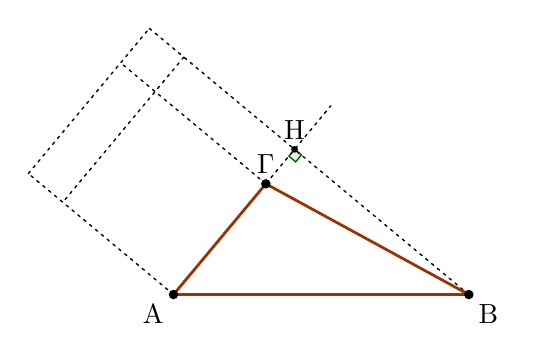
\begin{tikzpicture}[scale=.75]
\tkzSetUpLine[line width=1pt,color=black]
\tkzSetUpPoint[fill=black]

\tkzDefPoints{0/0/A,5/0/B,1.5625/1.875/C}

\tkzFillPolygon[fill=white](A,B,C)
\tkzDefPointBy[projection=onto A--C](B)\tkzGetPoint{H}

\tkzDefSquare(A,C) \tkzGetFirstPoint{A1} \tkzGetSecondPoint{A2}
\tkzDefSquare(A,H) \tkzGetFirstPoint{B1} \tkzGetSecondPoint{B2}

\tkzDefPointBy[projection=onto B1--B2](C)\tkzGetPoint{C1}
\tkzDefPointBy[projection=onto H--B1](A1)\tkzGetPoint{C2}

\tkzMarkRightAngles[line width=0.5pt, size=.15,color=AngleClr,fill=AngleClr,fill opacity=0.1](B,H,A)

\tkzDrawSegments[line width=0.5pt,color=black,dashed,dash pattern=on 1pt off 1.75pt](B,H B1,H C,C1 A,B2 B2,B1 C2,A2)
\tkzDrawSegments[line width=0.5pt,color=black,dashed,dash pattern=on 1pt off 1.75pt,add=0 and 0.3](A,H)

% \tkzDrawSegments[line width=0.5pt,color=black, add=0.4 and 0.4](B,H)

\tkzDrawPolygon[color=ShapeClr](A,B,C)
\tkzDrawPoints[size=3](A,B,C)
\tkzDrawPoints[size=2](H)
\tkzLabelPoint[below left](A){$\rm A$}
\tkzLabelPoint[below right](B){$\rm B$}
\tkzLabelPoint[above](C){$\rm \Gamma$}
\tkzLabelPoint[above](H){$\rm H$}

% \tkzMarkSegments[mark=s||,size=2.5](O,A O,B O,C)

\end{tikzpicture}

\end{document}
